% Data representation -- the ways a 3D airway tree can be stored, and where each is used here.
% Subsection of "Background", pulled in by sections/02-background.tex.
% The figure is generated by figures/make_airway_representations.py (synthetic tree).

\subsection{Data representation}         % how a 3D airway tree can be stored
\label{sec:data_representation}          % \secref{sec:data_representation}

A 3D pulmonary airway tree can be stored in several ways. The choice matters as it fixes what a
model sees (a volume, a surface, sample points or a skeleton), how much memory it needs, and
whether the branching structure is explicit or has to be inferred.
Figure~\ref{fig:airway_representations} shows the same tree in six common
representations, and Table~\ref{tab:airway_representations} summarizes their main properties.

\begin{figure}[htbp]                     % the six representations on one synthetic tree
  \centering                             % center the figure
  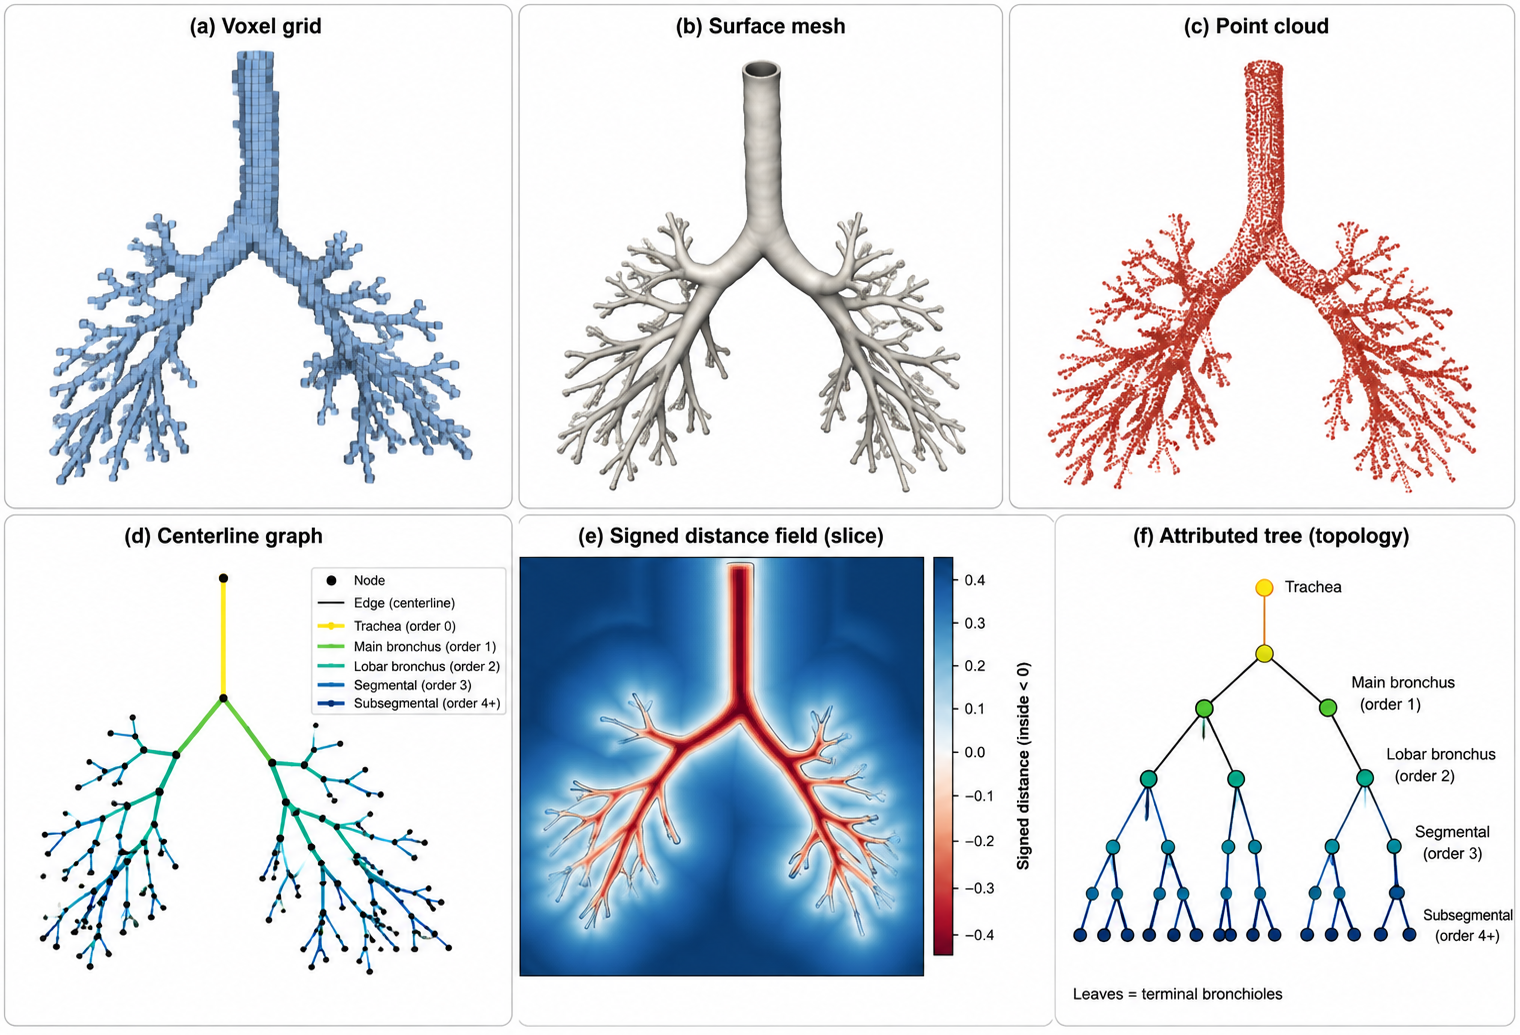
\includegraphics[width=\textwidth]{figures/airway_representations.png}  % made by figures/make_airway_representations.py
  \caption{The same synthetic airway tree (trachea and three generations) in six
           representations: (a) binary voxel grid, (b) triangulated surface mesh, (c) point
           cloud sampled on the surface, (d) centerline graph, with edge colour and width
           following the branch radius, (e) signed distance field on a slice through the first
           bifurcation, with the airway surface as the zero level set (black line), and
           (f) the abstract tree topology, whose edges carry attributes such as radius $r$ and
           length $\ell$.}
  \label{fig:airway_representations}     % referenced as Figure~\ref{fig:airway_representations}
\end{figure}

\paragraph{Voxel grid.}                  % (a) binary occupancy on a regular grid
The airway is a binary occupancy mask on a regular 3D grid, usually the grid of the CT scan
itself. This is the direct output of manual annotation and of segmentation networks, and the
format in which ATM'22 and AIIB23 are distributed (\secref{sec:datasets}). It fits 3D
convolutional networks naturally \cite{brock2016,garciauceda2021}, but memory grows with the
cube of the resolution while almost all voxels are empty, and the shape is limited by the voxel
spacing: thin distal branches cover only a few voxels and tend to look jagged or broken
\cite{zhang2024}. Sparse variants store only the occupied voxels, for example with the VDB
data structure \cite{museth2013} used by XCube \cite{ren2024}, or with sparse convolutions
\cite{prabhakar2026vaesselsparse}. In this work, voxel grids are used for registration
and by the dense and sparse autoencoders.

\paragraph{Surface mesh.}                % (b) triangulated lumen boundary
A surface mesh describes the boundary of the airway lumen with vertices and triangles. It is
usually extracted from the voxel mask with Marching Cubes \cite{lorensen1987}, or
reconstructed from points, e.g.\ by Poisson surface reconstruction in AVATREE
\cite{nousias2020avatree}. Meshes are compact, give sub-voxel smooth surfaces and are the
standard input for flow simulation \cite{lauria2022,ho2024}, but they carry no explicit branch
structure and can contain non-manifold elements, which is why their number is used as a
quality metric \cite{zhang2024}. In this work, meshes are extracted as the first step of the
implicit model's data preparation.

\paragraph{Point cloud.}                 % (c) unordered sample points
A point cloud is an unordered set of 3D points sampled on the surface of the airway tree. It
is sparse and independent of any grid, and it can be processed by point networks such as
PointNet++ \cite{qi2017} and Point Transformer \cite{zhao2021}. It has no connectivity, however,
so thin branches may receive too few points to be recognized. 
% In this work, IPGN samples
% foreground voxels as a point cloud, and the implicit model is trained on
% points sampled on and around the surface.

\paragraph{Centerline graph.}            % (d) skeleton as nodes and edges
Thinning the binary mask gives a one-voxel-wide skeleton \cite{lee1994,palagyi2006}, which can
be converted into a graph whose nodes are bifurcations and end points and whose edges are the
branches between them \cite{bumgarner2022}. Each edge can carry attributes such as radius,
length and direction. The representation is very compact and makes the branching topology
explicit, which is why it underlies most work on branch labeling
\cite{tschirren2005matching,feragen2011airway,xie2025}, morphometry
\cite{kaji2024airway,zhang2025airmorph} and graph generation \cite{prabhakar2024vesselgraph}.
Its weaknesses are its sensitivity to skeletonization artefacts, such as spurious short branches,
and the loss of the lumen shape beyond the stored attributes. In this work, the centerline
graph is an input of IPGN - the model that used to generate the labels - and the basis of the morphological
descriptors.

\paragraph{Implicit function.}           % (e) zero level set of a continuous field
The surface can also be defined as the zero level set of a continuous function of space,
typically a signed distance field (SDF) that is negative inside the airway and positive
outside. Neural implicit representations learn this function with a small network conditioned
on a latent code \cite{park2019,sitzmann2020}, or store it in feature planes that can be queried
anywhere \cite{weng2026topofield}. The result is continuous, resolution-free and smooth, but a
mesh has to be extracted to visualize it, and the topology is not explicit; DGCI addresses this
by learning correspondences through a space shared by all trees \cite{zhang2024}. In this work,
the implicit representation is the one that produced the best reconstructions.

\paragraph{Attributed tree and parametric models.}  % (f) abstract topology with attributes
Finally, the airway can be reduced to a combinatorial tree whose edges carry geometric
attributes, such as radius, length or landmark points along the branch. Idealized airway
models describe the whole tree this way \cite{horsfield1971models,kitaoka1999}, tree-shape
spaces use it to compare and average trees \cite{feragen2011means,feragen2011airway}, and
generative models encode it recursively \cite{feldman2023vesselvae,batten2025vetta} or as a
sequence of nodes \cite{feldman2025vesselgpt}. Branch geometry can in turn be described
parametrically, e.g.\ with NURBS \cite{ortizpuerta2022} or B-spline cross-sections
\cite{feldman2025vesselgpt}. Such representations are compact and interpretable, but they
depend on a reliable extraction of the tree, and trifurcations or loops break the assumption of
a binary tree \cite{miyawaki2017automatic}. The morphological descriptors used in this work
operate on such a tree, whose nodes carry an anatomical label, a generation number and a length.

\begin{table}[htbp]                      % side-by-side comparison of the representations
  \centering                             % center the table
  \small                                 % slightly smaller font so the table fits
  \caption{Main properties of the airway tree representations, and where each one is used in
           this work.}
  \label{tab:airway_representations}     % referenced as Table~\ref{tab:airway_representations}
  \begin{tabular}{llcl}                  % name, geometry, explicit branching, use here
    \toprule
    Representation   & Geometry            & Branching explicit & Used in this work \\
    \midrule
    Voxel grid       & Discrete volume     & No  & Registration, VAE, autoencoders \\
    Sparse voxels    & Occupied voxels     & No  & Sparse encoder \\
    Surface mesh     & Continuous surface  & No  & Implicit model (data preparation) \\
    Point cloud      & Sampled points      & No  & Labelling (IPGN), Implicit model \\
    Centerline graph & 1D skeleton         & Yes & Labelling (IPGN), morphological metrics \\
    Implicit (SDF)   & Continuous field    & No  & Implicit encoding (DGCI) \\
    Attributed tree  & Abstract topology   & Yes & Morphological metrics \\
    \bottomrule
  \end{tabular}
\end{table}
